\section{Discussion}

% \begin{figure}
\begin{center}

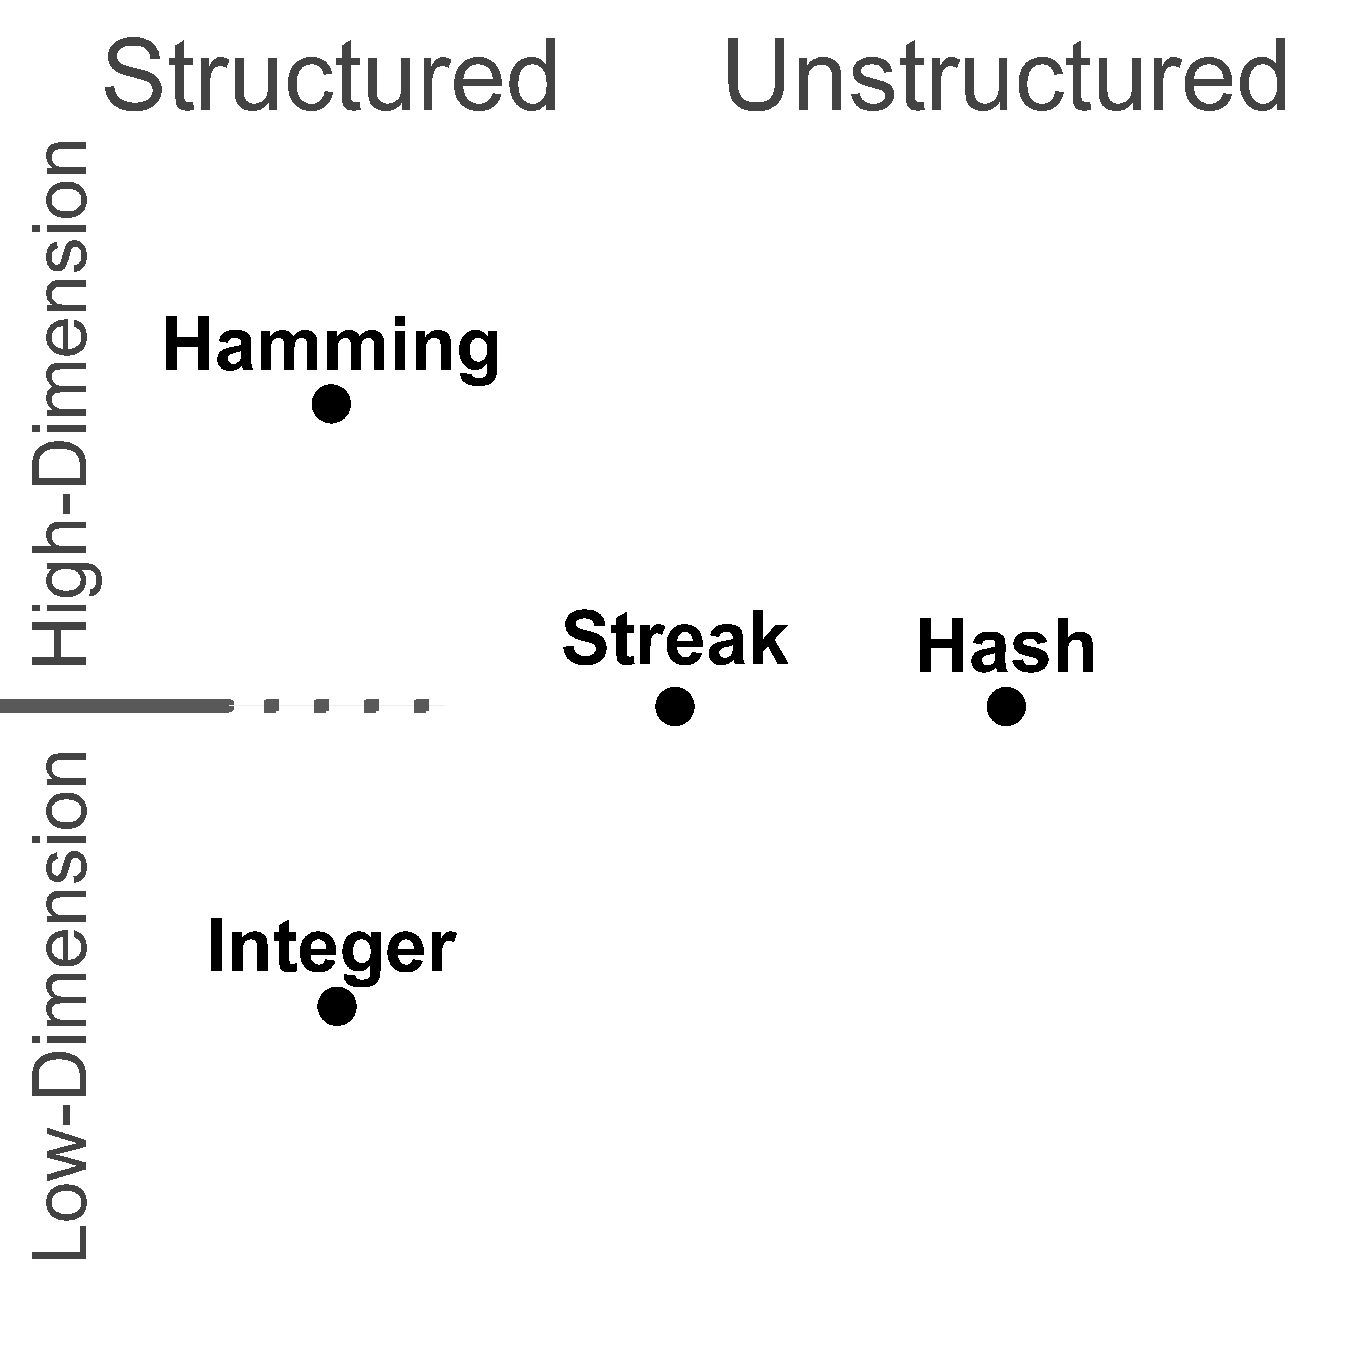
\includegraphics[width=\columnwidth]{img/conceptual-geometry}
\caption{
A conceptual schematic of the tag-matching metrics' geometric properties.
}
\label{fig:conceptual_geometry}

\end{center}
\end{figure}

First, we performed geometrical analyses to understand how our panel of tag-matching metrics constrain the patterns of that tend to, or even are possible to, arise.
If two tags both closely match a third tag, will these two tags be constrained to closely match each other?
Likewise, if a tag closely matches a second tag, will the tag be constrained to poorly match other tags the second tag poorly matches?

We found that the bidirectional integer metric exhibited the tightest geometrical constraint in our analyses.
The unidirectional integer metric also exhibits tight geometrical constraint, but quirks of its non-commutative construction allows that constraint to split across extremes of poor- and close-matching.
Hamming and streak metrics are more loosely constrained, with the streak metric allowing for edge cases that very strongly break geometric constraint.
Finally, the hash metric exhibits no geometrical structure or constraint.

Next, we analyzed the effect of bitwise mutation on match distance score under the different metrics.
Under the hamming metric, all mutations have small effects on match distance score.
In contrast, under the integer metrics, rare mutations have strong effects on match distance score.
The streak metric also exhibited strong-effect mutations, particularly on coupling loosely-affiliated tags.
The hash metric exhibited the fattest tails of mutational effect, with strong-effect mutations occuring frequently.
Interestingly, the hash metric also exhibited sign-outcome frequencies that differed from the other metrics.
Mutations that decoupled tightly-matching tags and mutations that coupled loosely-matching tags were more frequent.

On mutational walks from an identical tag pair, the hamming metric exhibited the greatest robustness to mutation, followed by the streak metric.
The integer metrics, in particular the unidirectional integer metric, exhibted less robustness.
The streak metric, where all one-step mutations scramble match distance, exhibited the least robustness.

In target-matching evolutionary experiments, we found that the hash metric enabled rapid adaptive evolution towards targets with low tag-matching constraint.
This rapid evolution may be due to the hash metric's ability to rapidly generate variation.
In cases with high tag-matching consraint, however, the hash metric yielded poor-quality solutions.
The integer metrics also yielded poor-quality solutions for targets with tag-matching constraint.
In some more-constrained cases, the streak metric enabled more rapid adaptive evolution than the hamming metric.

In evolutionary experiments to evolve genetic programs, we found that the hamming and streak metrics yielded successful solutions the most frequently.
The hash metric had the next best performance, yielding more solutions than the integer metrics, which performed comparably.
Interestingly, on the directional signal task, which tends to evolve networks with more tag-matching constraints (high-degree regualation/activation interaction network) we found evidence that the streak metric enabled more rapid adaptive evolution than the hamming metric.

The streak metric seems to offer variational and geometric properties that are in many ways intermediate between the hash metric and the integer and hamming metrics.
It exhibits low, but some, geometric constraint.
Many mutations are neutral (like the integer metrics) but extreme-effect mutations also occur.
However, it is unclear exactly why it enabled more rapid adaptive evolution on the genetic programming problem.



